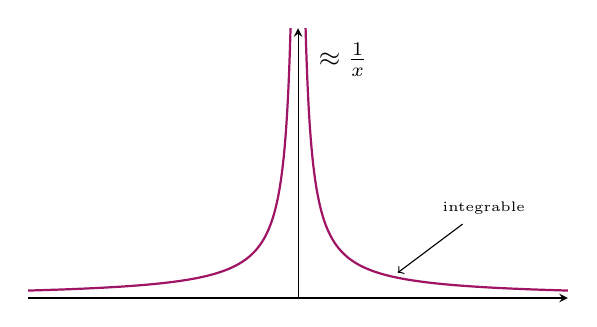
\begin{tikzpicture}
 \begin{axis}[
 	unit vector ratio*=1 1 1,
	axis lines = middle,
	ytick=\empty,
	xtick={0},
	xticklabel={0},
	scaled ticks = false,
	xmin = -6,
	xmax = 6,
	ymin = 0,
	ymax = 6,
	]
	\addplot[
	RedViolet, 
	thick, 
	domain = 0:20,
	samples=1000, 
	]
	{1/x};
	\addplot[
	RedViolet, 
	thick, 
	domain = 0:-20,
	samples=1000, 
	]
	{abs(1/x)};
	\node [anchor=west](source) at (axis cs:3,2) {\tiny integrable};
	\node (destination) at (axis cs:2,0.4){};
	\draw[->](source)--(destination);
	\node(lol) at(axis cs:1,5.3) {$\approx\frac{1}{x}$};
\end{axis}
\end{tikzpicture}